\documentclass[conference]{IEEEtran}
\usepackage{cite}
\usepackage{amsmath,amssymb,amsfonts}
\usepackage{algorithmic}
\usepackage{graphicx}
\usepackage{textcomp}
\usepackage{xcolor}
\usepackage{tikz}
\usetikzlibrary{positioning}
\graphicspath{{./images/}}

\def\BibTeX{{\rm B\kern-.05em{\sc i\kern-.025em b}\kern-.08em
    T\kern-.1667em\lower.7ex\hbox{E}\kern-.125emX}} 
% Preamble for page numbering

\begin{document}

\title{On Wireless Audio: A Brief Literature Review}

\author{\IEEEauthorblockN{Diego Cruz}
    \IEEEauthorblockA{\textit{Dept. of Computer Engineering} \\
        \textit{San Jose State University}\\
        San Jose, United States \\
        diego.cruz@sjsu.edu}
    \and
    \IEEEauthorblockN{Shiv Shankar Yadav}
    \IEEEauthorblockA{\textit{Dept. of Computer Engineering} \\
        \textit{San Jose State University}\\
        San Jose, United States \\
        shivshankar.yadav@sjsu.edu}
    \and
    \IEEEauthorblockN{Mahima Agumbe Suresh}
    \IEEEauthorblockA{\textit{Dept. of Computer Engineering} \\
        \textit{San Jose State University}\\
        San Jose, United States \\
        mahima.agumbesuresh@sjsu.edu}
}

\maketitle

\begin{abstract}
    This literature review provides an intermediate overview of
    different wireless audio technologies, spanning the historical evolution and
    contemporary advancements in the field. The review
    begins with a basic history of wireless communications spanning from
    the Marconi wireless telegraph to the modern establishment of
    Bluetooth and 802.11 Wi-Fi as IEEE standards for wireless
    communications at different scales. From there, different
    technologies such as Radio Frequency, Infrared, Bluetooth, 802.11
    Wi-Fi, Near-Field Communication, and AptX/LDAC are explored with one
    particular application/configuration and/or evaluated based on their
    particular use cases. The literature review concludes with a
    forward-looking point of view, taking insight from a dialogue with a
    professional audio engineer, providing the perspective of possible end users on the
    trajectory of wireless audio as a medium. This particular literature
    review is intended as a valuable resource for SJSU Students to learn
    the basics of wireless audio leading up to the time at which this
    paper was published, as well as the larger communities spanning
    researchers, engineers, and audio enthusiasts respectably working to
    understand the constantly-evolving dynamic scape of wireless audio.
\end{abstract}

\begin{IEEEkeywords}
    Wireless Audio, Fidelity, Wireless Networks, Bluetooth, 802.11 Wi-Fi
\end{IEEEkeywords}

\section*{Introduction}
Wireless audio is not particularly a new technology, but there have been several different
implementations such as radio waves, Bluetooth audio, and proprietary protocols that
private corporations have made for their respective products.\cite{bhalla_unraveling_2021}
Modern research has included the possibility of using end-to-end audio transmission using
laser communications \cite{anthony_approach_2021}, or otherwise creating hybridizations
between Wi-Fi and Bluetooth audio implementations to minimize interference.
\cite{forenbacher_throughput_2021}

The most well-recognized wireless audio protocol today is the Bluetooth audio protocol
or the IEEE 802.11 WiFi protocol, but there exist different methods and protocols
such as broadcast radio, Apple's native AirPlay, and the Digital Living Network
Alliance (DLNA) standards suite among several others.\cite{parks_wireless_2013}

The intention of this literature review is to investigate the realm of wireless local area
networks at a small scale. The different protocols and technologies/standards
surrounding wireless audio often are constrained to scales built on line of sight,
but some stand out among others to cover different rooms within a building.
However, there will naturally be a brief review of the history of wireless
communications regarding strictly the transmission and reception of audio
signals, or other signals that are then transcribed to audio.

\section*{The History of Wireless Audio}
To understand the history of wireless audio, one must first understand the history of
wireless communications. In general, wireless communications were developed from a need to
communicate across vast distances without the logistical nightmare of cabling across various
environments. A few realworld examples could include having to transmit signals across
mountain ranges, or having to communicate between land and sea, and perhaps between
continents at large.\cite{noauthor_ericsson_2001} Ultimately, the one given the most credit
for inventing modern wireless communication began with Guglielmo Marconi developing the
wireless telegraph, which was capable of utilizing radio frequencies to send Morse code
messages across vast distances. His hallmark demonstration was in sending a wireless Morse
code transmission from the United Kingdom to Canada.\cite{noauthor_ericsson_2001}

Following innovations in communications hardware such as the triode and the vacuum tube
receiver/transmitter\cite{white_pre-war_2003}, the Marconi telegraph led to the invention of
the radio, resulting in a mass adoption of the radio in the American household.\cite
{noauthor_ericsson_2001} During the 1950s, only then were wireless telephones made more
common with systems like the Ericsson MTA vehicular telephony system. A few decades later,
nearing the end of the Cold War, the GSM specifications established in the 90s
\cite{suresh_introduction_2023}, there were increasingly compact telephones capable of
fitting in the pocket of an individual.\cite{noauthor_ericsson_2001}

It is around this time that Ericsson, a communications company that specialized in telephony,
began to explore avenues of communication surrounding the personal computer, eventually
leading to the creation of the first Bluetooth specification in the late 90s and brought to
market in 2001.\cite{irekvist_bluetooth_2022} Later on, IEEE would modify their 802.11
specification to include Bluetooth audio as well as an wireless audio implementation native
to the Wi-Fi protocol.\cite{noauthor_bluetooth_nodate}

\section*{Discussion}

A few studies have been chosen for the purposes of this particular literature review, to
showcase and display different technologies that were used for wireless audio at some point.
The aforementioned technologies are listed below:

\begin{itemize}
    \item Radio Frequency (RF)
    \item Infrared (IR)
    \item Bluetooth (BT)
    \item 802.11 Wi-Fi Audio
    \item Near-Field Communication (NFC)
    \item AptX and LDAC
\end{itemize}

% Insert RF tidbit here, above the blurb I typed in IR
Lorem ipsum dolor sit amet, consectetur adipiscing elit. Quod cum accidisset ut alter alterum
necopinato videremus, surrexit statim. Videamus igitur sententias eorum, tum ad verba
redeamus. Duo Reges: constructio interrete. Quam ob rem tandem, inquit, non satisfacit? Res
enim se praeclare habebat, et quidem in utraque parte. Quae tamen a te agetur non melior,
quam illae sunt, quas interdum optines. Earum etiam rerum, quas terra gignit, educatio
quaedam et perfectio est non dissimilis animantium. Alterum significari idem, ut si
diceretur, officia media omnia aut pleraque servantem vivere. Id enim natura desiderat.
Quamquam ab iis philosophiam et omnes ingenuas disciplinas habemus;

% IR portion
With respect to infrared audio transmission, a small group of researchers developed an
approach to end-to-end audio transmission using laser communications in 2021. The methodology
of the study involved the use of small-scale hardware to simulate the transmission and
reception of audio signals at a larger scale, and the use of software to enable the hardware
to align to maximize throughput. The transmitter of the small-scale system was composed of a
microcontroller, a rotating sensor to align the transmitting laser with the receiver, a
modulation circuit to encode the audio input, and a transmitting laser to send the signal.
And, the receiver of the system was composed of an alignment laser that would align with the
rotating sensor of the transmitter, a photodiode that would take in the transmitting laser,
and a demodulation circuit to decode the audio. The overall hardware architecture has been
depicted as shown in Figure~\ref{fig:IR_hardware}.\cite{anthony_approach_2021}

\begin{figure}[htbp]
    \centering
    \includegraphics[width=1\linewidth]{anthony-et-al-diagram.jpg}
    \caption{IR Audio Hardware Architecture \cite{anthony_approach_2021}}
    \label{fig:IR_hardware}
\end{figure}

In the context of that area of study, it has been established that laser communications are
less susceptible to signal interference because of the relative lack of cross traffic that
could result in signal or data loss.Additionally, the signal itself does not require any kind
of shielding whereas wired communications would need some sort of protection over long
distance transmissions. However, this does not mean that IR wireless audio is without its
shortcomings, as it is heavily dependent on the transmitter and receiver having a 'line of
sight' towards each other, which means that there would be a point where the distance would
be too great due to the curvature of the earth itself. Laser communications finds itself as a
useful technology between short and midrange distances for signals which require high
fidelity, while RF is particularly useful for long-range communications where reach is
considered more important than fidelity.\cite{anthony_approach_2021}

% Bluetooth Portion
With respect to Bluetooth, the specifications of IEEE standards will be referenced, which
refers to version 1.1 until version 4.0, and the Bluetooth Special Interest Group (SIG) has
managed Bluetooth from version 4.0 to its current iteration: 5.4. Bluetooth seldom needs an
introduction, as it is one of the most ubiquitous forms of wireless audio for consumer-grade
electronics. As previously mentioned, it was adopted in 2001-2002 as IEEE 802.15.1 but is no
longer actively maintained by IEEE.\cite{bhalla_unraveling_2021} Even then, Bluetooth has an
extensive history with the IEEE with a multitude of updates that prioritize
backwards-compatibility, similar to the Intel x86 processor architecture.
\cite{noauthor_bluetooth_nodate} As such, we will first examine the development of Bluetooth
over time as well as explore Bluetooth Low-Energy, otherwise known as Bluetooth LE.
\cite{bhalla_unraveling_2021}

Bluetooth is a short-range wireless communications protocol that can range between 10-15
meters, depending on the version that is implemented into the device. It is used for
different applications, including abstract data transmission as well as audio transmission.
Bluetooth typically makes use of radio frequencies spanning 2400 MHz to 2483 MHz, and is at
its core, a packet-based protocol that sends packets over 79 channels that are chosen
seemingly at random. These 79 channels are cycled at a capacity of 1600 times per second.
This 'hopping' technique is known as Frequency Hopping Spread Spectrum (FHSS), which could be
used as a security measure because it is capable of encrypting audio. However, Bluetooth
relies on additional encryption using private keys for each party and are only known to the
devices involved with each other. Over the years, Bluetooth has seen different changes such
as modifications to its FHSS or enhancements to its throughput, known as Enhanced Data Rate
(EDR), or changes to its medium access protocols (MACs) otherwise known as Alernative MAC/
PHY (AMP). Ultimately, leading up to Bluetooth 4.0 in 2010, changes based on contemporary
Wi-Fi implementations and refinements to legacy protocols had been made under the oversight
of IEEE.\cite{noauthor_bluetooth_nodate}

\begin{figure}
    \centering
    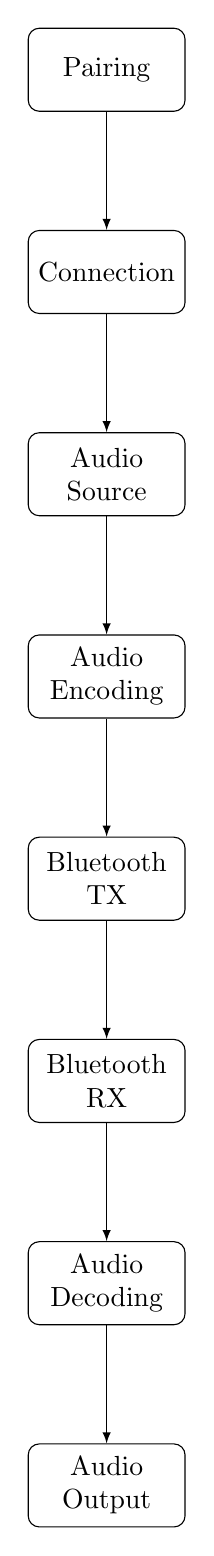
\begin{tikzpicture}[node distance=1.5cm, auto, block/.style={rectangle, draw, text width=5em, text centered, rounded corners, minimum height=3em}, line/.style={draw, -latex}]
        % Nodes
        \node [block] (pairing) {Pairing};
        \node [block, below=of pairing] (connection) {Connection};
        \node [block, below=of connection] (source) {Audio Source};
        \node [block, below=of source] (encoding) {Audio Encoding};
        \node [block, below=of encoding] (transmission) {Bluetooth TX};
        \node [block, below=of transmission] (reception) {Bluetooth RX};
        \node [block, below=of reception] (decoding) {Audio Decoding};
        \node [block, below=of decoding] (output) {Audio Output};

        % Arrows
        \path [line] (pairing) -- (connection);
        \path [line] (connection) -- (source);
        \path [line] (source) -- (encoding);
        \path [line] (encoding) -- (transmission);
        \path [line] (transmission) -- (reception);
        \path [line] (reception) -- (decoding);
        \path [line] (decoding) -- (output);
    \end{tikzpicture}
    \caption{Bluetooth Audio Transmission Process}
    \label{fig:bluetooth_process}
\end{figure}

Past 2010, under the supervision of SIG, Bluetooth LE was established which operates under a
similar premise compared to conventional Bluetooth, but was different in that it had
energy-saving measures to help battery-powered devices last for a long time. This is
accomplished by having the device in sleep mode for most of the time until communication was
established from the 'host' devices.\cite{bhalla_unraveling_2021} Bluetooth LE makes use its
unique data advertising for device discovery and connection, which can further be used to
advertise general application data to an unlimited number of listeners. LE is not directly
compatible with conventional bluetooth, but both implementations can be physically applied to
the hardware so it can use either one.\cite{bhalla_unraveling_2021} In regards to the radio
frequencies used, LE makes use of 40 channels that are hopped with FHSS at slower rates to
conserve power, which can enable multiple exchanges while on the same channel.
\cite{noauthor_bluetooth_nodate} This particular technology sees frequent use in wireless
audio, because specializations were made that allowed for a consistent exchange while
conserving energy and thus prolonging battery life.\cite{bhalla_unraveling_2021}

% Insert 802.11 WiFi Audio tidbit here 
Lorem ipsum dolor sit amet, consectetur adipiscing elit. Quod cum accidisset ut alter alterum
necopinato videremus, surrexit statim. Videamus igitur sententias eorum, tum ad verba
redeamus. Duo Reges: constructio interrete. Quam ob rem tandem, inquit, non satisfacit? Res
enim se praeclare habebat, et quidem in utraque parte. Quae tamen a te agetur non melior,
quam illae sunt, quas interdum optines. Earum etiam rerum, quas terra gignit, educatio
quaedam et perfectio est non dissimilis animantium. Alterum significari idem, ut si
diceretur, officia media omnia aut pleraque servantem vivere. Id enim natura desiderat.
Quamquam ab iis philosophiam et omnes ingenuas disciplinas habemus;

% Insert NFC and AptX/LDAC tidbit here
Lorem ipsum dolor sit amet, consectetur adipiscing elit. Quod cum accidisset ut alter alterum
necopinato videremus, surrexit statim. Videamus igitur sententias eorum, tum ad verba
redeamus. Duo Reges: constructio interrete. Quam ob rem tandem, inquit, non satisfacit? Res
enim se praeclare habebat, et quidem in utraque parte. Quae tamen a te agetur non melior,
quam illae sunt, quas interdum optines. Earum etiam rerum, quas terra gignit, educatio
quaedam et perfectio est non dissimilis animantium. Alterum significari idem, ut si
diceretur, officia media omnia aut pleraque servantem vivere. Id enim natura desiderat.
Quamquam ab iis philosophiam et omnes ingenuas disciplinas habemus;

% Future technology and correspondence portion
In addition to the previously discussed technologies, there are emergent audio technologies
that are pushing the envelope of wireless high-fidelity (Hi-Fi) audio. One such technology
involves a proprietary wireless communication standard that is capable of transmitting audio
at a 16ms latency: The AIAIAI Audio UNIT-4 Wireless+ speakers with the W+ Link technology.
This particular technology does not have publicly available specifications, but AIAIAI have
stated some of the key differences that distinguishes it from bluetooth. One such difference
is that the W+ Link technology makes use of two antennas for reception and transmission of
information as opposed to the singular antenna that Bluetooth makes use of. What the presence
of two antennas entail is the ability to swap between one or the other if one connection
drops out. Additionally, the technology prioritizes keeping the same latency by means of
swapping between pre-defined radio frequency bands as opposed to using a pseudorandom
pattern. Additionally, the W+ Link technology does not compress audio, delivering it at a 44.
1 kHz 16-bit quality, roughly equating to a little over 1400 Kbps.\cite{noauthor_unit-4_2023}

\begin{figure}[htbp]
    \centering
    \includegraphics[width=1\linewidth]{Unit-4_wireless_showcase.jpg}
    \caption{AIAIAI UNIT-4 Wireless+ \cite{noauthor_unit-4_2023}}
    \label{fig:unit-4_productPic}
\end{figure}

\subsection*{A Correspondence with an Audio Engineer}

To gather more information about the UNIT-4 Wireless+ as well as the perspective of prospective end users, the authors of this work reached out to Michael Wynne, who is currently a professional audio mastering engineer but has done work as a producer, audio recording engineer, and as an audio mixing engineer. Mr. Wynne has done extensive work providing free education about music/audio production on his YouTube Channel "In The Mix." \cite{wynne_i_nodate}

\begin{figure}[htbp]
    \centering
    \includegraphics[width=1\linewidth]{Michael_In-The-Mix.jpg}
    \caption{Michael Wynne, with his dog, Solo}
    \label{fig:in-the-mix_portrait}
\end{figure}

Below is the unedited online correspondence:

\subsubsection*{Question 1}
\textbf{Q:} What is your experience in the world of audio engineering. Were you formally
taught at an institution, did you attend some classes, or did you teach yourself with
experimentation and the internet??

\textbf{A:} While I have no formal education in music production or mixing, I have had a few
mentors along the way and have learned through experience on the job. There are many good
resources online and I find that taking them all on balance is a good approach. Not relying
on only 1 or 2 sources of information.

\subsubsection*{Question 2}
\textbf{Q:} Before you published the video on the Unit-4 Wireless+ loudspeakers, did you have
any experience with wireless audio, including consumer and higher-grade materials? (e.g. Car
radio, internet calls, Bluetooth, Wi-Fi audio, etc.)


\textbf{A:}  I have used wireless audio devices for as long as I can remember, portable
speakers, headphones, car stereos etc. I have not studied wireless protocols deeply but did
feel that the current offerings were not utilising the most recent advancements in Bluetooth
technology.

\subsubsection*{Question 3}
\textbf{Q:} Adding on to the previous question, do you have any experience with opening up
loudspeakers, headphones, or any audio hardware to perform repairs or intermediate/advanced
maintenance?

\textbf{A:} I have luckily not needed to do repairs on any hardware (in almost 7 years, I
guess I'm lucky!) but I have opened up or taken apart almost everything I use besides my PSI
A23m and my power conditioner.

\subsubsection*{Question 4}
\textbf{Q:} In your opinion, do you think that the Unit-4 wireless+ loudspeakers will be
something of a market exception in high-fidelity audio, or do you think it has the potential
to establish a new trend in loudspeakers?

\textbf{A:}  I think it's the first in a new class. It will not be long before many other
companies produce a practical wireless system. The lack of wires has been so much more
helpful than I expected. I regularly use them as high-quality hi-fi speakers in the lounge, I
take 1 into the kitchen when cooking etc and they sound so much better than my other
Bluetooth speakers. However, the other Bluetooth speakers I have are \$150 and less so it is
not a fair comparison!

\subsubsection*{Question 5}
\textbf{Q:} With respect to your comments made on latency (namely the 16ms figure), something
I'd like to add on to that is that loudspeakers in general have some components in them that
perform analog to digital (and vice-versa) conversion on output AND input which results in
some latency right out the gate (typically in the ballpark of 5 to about 12ms).

With this in mind, do you think that latency will still be the factor that keeps most
prospective users away from wireless high-fidelity audio, or do you think there is something
else at play that would encourage end users to seek out conventional wired solutions?

\textbf{A:} Yes, this is something I didn't make clear in the video. Many people claimed that
they required 0ms latency (which practically does not exist, certainly not within most of our
budgets and computing constraints...). I think the latency will keep people away until they
try them. I was initially put off by the latency but told AIAIAI to send a pair over for me
to test anyway. As it turned out, the latency was a complete non-issue. I literally cannot
feel or hear the latency when recording.

\subsubsection*{Question 6}
\textbf{Q:} While you covered the loudspeaker design (including the dynamic drivers) while
performing the teardown in the video, are there any physical designs that you think would be
interesting when paired with wireless audio technologies? (e.g. Planar Magnetic Drivers,
Electrostatic Drivers, etc.)

\textbf{A:} Certainly. I think it makes sense to keep the designs cheaper, rugged and more
simple to start off with but I would like to see many more technologies employed.
My initial thought when using the speakers was to use them for Dolby atmos. with slightly
more battery power, it would negate the need to run audio and power cables x12 all over the
room, walls and ceilings. \cite{wynne_interviewing_2023}

\section*{Conclusion and Future Work}

Reflecting on the history of wireless audio as well as the inner workings of the different
related technologies over the years, the authors intend to remind you, the reader, that the
central problem has always been surrounding the ability of humans to connect with one
another, regardless of geography or socioeconomic stability. With battery, charging, and
wireless technology having evolved at such a rapid pace within the previous 20 years, there
may yet be a wireless renaissance wherein old designs are given new life because much more
can be packed into form factors of days past. To elaborate, modern wireless audio hardware is
easily able to pack much more punch because less real estate and energy resources are used
toward the writing/reading technologies of CD Boomboxes or Cassette players, and are
substituted by a few chips using Bluetooth or some specially-made wireless communication
protocol.

The authors provide full permissions for any future SJSU Students to build upon the work and
create an updated literature review of wireless audio, so long as proper citations are
provided. All assets will be provided and made free so long as the project supervisor is
willing to host the information over some file sharing medium.

\vfill
\bibliographystyle{IEEEtran}
\bibliography{cmpe189}

\vspace{12pt}
\end{document}
